\chapter*{前言与阅读路线}
\markboth{\sffamily\slshape 前言}
{\sffamily\slshape 前言}


扩散模型已迅速成为生成建模的核心范式，其大量工作涵盖机器学习、计算机视觉、自然语言处理等领域。这些文献分散在各个社区中，并强调了不同方面的进展，包括涉及建模原理、训练目标、采样器设计及其背后的数学思想的理论基础；涵盖工程实践和架构选择的实施进展；使模型适应特定领域或任务的实际应用；以及提高计算、内存和部署效率的系统级优化。本书旨在提供一个 \emph{原则基础} 扩散模型，重点关注以下中心主题：
\begin{itemize}
    \item 我们提出了锚定扩散模型研究的基本概念和公式，为读者提供了导航更广泛文献所需的核心理解。我们不会调查所有变体或特定领域的应用程序；相反，我们建立了一个稳定的概念基础，从中可以理解这些发展。
    \item 与学习从噪声到数据的直接映射的经典生成模型不同，扩散模型将生成视为随着时间的推移逐渐转变，将粗糙的结构细化为精细的细节。这一中心思想是通过三个主要视角来发展的，即 \emph{变体}, \emph{基于分数}、 和 \emph{基于流} 方法，提供理解和实现扩散建模的补充方法。我们专注于这些公式的核心原则和基础，旨在追溯其关键思想的起源，阐明不同公式之间的关系，并形成将直观洞察力与严格数学公式联系起来的连贯理解。
    \item 在此基础上，我们研究了如何进一步开发扩散模型，以更有效地生成样本，提供对生成过程的更大控制，并激发基于扩散原理的独立形式的生成建模。
\end{itemize}


本书面向对深度学习（例如，神经网络是什么以及训练如何工作），或更具体地说，深度生成建模有基本了解，并且希望加深对扩散模型超越表面熟悉程度的理解的研究人员、研究生和从业者。到最后，读者将对扩散模型的基础有一个原则性的理解，在一个连贯的框架内解释不同公式的能力，以及自信地应用现有模型和追求新的研究方向所需的背景。









\section*{\centering \Large 本书路线图}

本书系统地介绍了扩散模型的基础，并将其追溯到其核心基本原理。

\paragraph{建议阅读路径.}  
我们建议按照所示顺序阅读本书，以建立全面的理解。已经熟悉基础知识的读者可以跳过标记为 \emph{Optional} 的部分。例如，那些熟悉深度生成模型 (DGM) 的人可能会绕过 \Cref{ch:overview-dgm} 中的概述。同样，变分自编码器 (\Cref{sec:vae})、能量模型 (\Cref{sec:ebm}) 或归一化流 (\Cref{sec:flow-based-method}) 的先验知识允许跳过这些介绍性部分。其他可选部分提供对高级或专业主题的更深入的见解，可以根据需要进行咨询。

本书分为四个主要部分。
\paragraph{A 部分 \& B：扩散模型的基础.}
本节通过回顾塑造该领域的三个基本观点来追溯扩散模型的起源\footnote{我们指出，我们对扩散的三个观点的组织
模型是概念性的而不是时间顺序的。例如，
\emph{ 基于能源的方法 } 有着悠久的历史。
统计力学将概率与能量联系起来，而研究
布朗运动和后续工作描述了概率如何
分布随着时间的推移而演变
~\citep{gibbs1902elementary,langevin1908brownian,fokker1914mittlere,planck1917satz,kolmogorov1931}。现代扩散概率论
模型后来将相关思想带入生成建模中并
明确地从非平衡统计物理学中汲取灵感
~\citep{sohl2015deep}。这里提出的三个观点
因此应该被理解为解释扩散的现代方式
模型，而不是作为其所在位置的严格历史排序
基本思想首先出现。}。 \Cref{fig:part-b-roadmap} 提供了这部分的概述。

\subparagraph{A 部分：深度生成建模 (DGM) 简介.}
我们从 \Cref{ch:overview-dgm} 开始回顾深度生成建模的基本目标。从数据示例集合开始，目标是构建一个模型，该模型可以生成新示例，这些新示例似乎来自相同的底层且通常未知的数据分布。许多方法通过学习数据的分布方式来实现这一点，要么显式地通过概率模型，要么隐式地通过学习的转换。然后，我们解释这些模型如何用神经网络表示数据分布，它们如何从示例中学习，以及它们如何生成新样本。本章最后对主要生成框架进行了分类，强调了它们的中心思想和主要区别。








\subparagraph{B 部分：扩散模型的核心观点.}\begin{figure}[th!]
\vspace{-0.5cm}
    \centering
    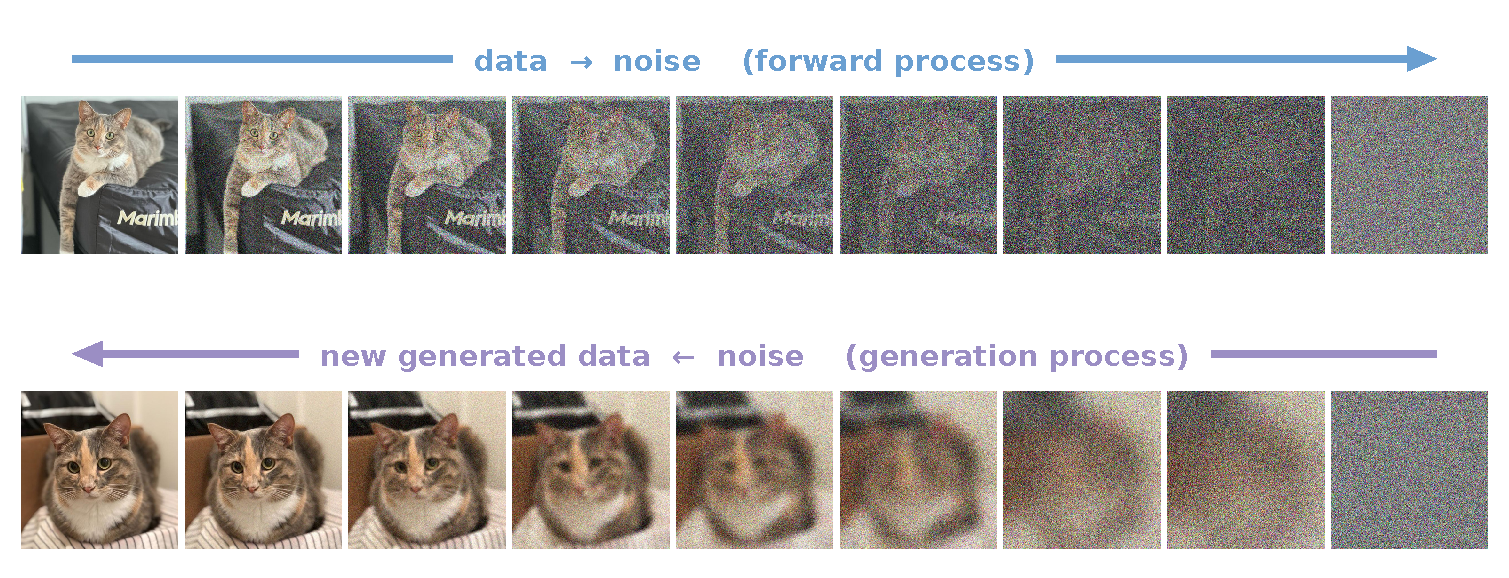
\includegraphics[width=\linewidth]{Images/PartA/diffusion_forward_vs_reverse.pdf}
    \caption{\textbfs{前向和反向扩散轨迹。} 在前向过程（顶部）中，真实数据样本逐渐被噪声破坏，通过一系列中间噪声阶段，直到它与纯噪声无法区分。在相反的过程中（底部），生成从新的噪声样本开始，并逐渐消除噪声以生成新图像。相反的过程并不是重建训练期间看到的特定示例。相反，它从新鲜的噪音开始，逐渐将其塑造成现实的新样本。 \figcredit{由作者创建。}}
    \label{fig:ill-forward-reverse}
\end{figure}

概述了深度生成建模的总体目标和机制后，我们现在转向扩散模型，这是一类将生成实现为从噪声到数据的逐步转换的方法（参见 \Cref{fig:ill-forward-reverse}）。核心思想很简单：通过添加噪声可以逐渐破坏数据样本，直到它与纯粹的随机性无法区分。这个\emph{前向过程}将不同的数据样本移动到相同的简单噪声空间中，这很容易从中采样并作为生成的起点。在此过程中，它还创建了连接数据和噪声的中间噪声阶段的平滑序列。为了生成，我们从这个空间中抽取一个新的噪声样本，并通过 \emph{ 逆时（生成）过程 } 逐渐消除噪声，最终产生一个新的数据样本。这一逆向过程并不能恢复某个特定的原始示例；相反，它从新鲜的噪音开始，逐渐将其转化为现实的数据。我们研究了三个相互关联的框架，每个框架都建立在相同的原理上：一个逐渐增加噪声的正向过程，以及一个由逐渐去噪的模型序列近似的逆时过程：
\begin{itemize}
    \item \textbfs{变分视图}（\Cref{ch:variational}）：源自变分自编码器（VAE）~\citep{kingma2013auto}，它将扩散框架为通过变分目标学习去噪过程，从而产生去噪扩散概率模型(DDPM)~\citep{sohl2015deep,ho2020denoising}。
    \item \textbfs{基于评分的视图} (\Cref{ch:score-based})：植根于能量模型(EBM)\\~\citep{ackley1985learning}，并发展为噪声条件分数网络(NCSN)~\citep{song2019generative}。它学习分数函数，即日志数据密度的梯度，指导如何逐步去除样本中的噪声。在连续时间内，\Cref{ch:score-sde} 引入了 \emph{Score SDE 框架}，该框架将这种去噪过程描述为随机微分方程（SDE），并将其确定性对应物描述为常微分方程（ODE）。这种观点将扩散建模与经典微分方程理论联系起来，为分析和算法设计提供了清晰的数学基础。\item \textbfs{基于流的视图} (\Cref{ch:flow-based})：基于归一化流~\citep{rezende2015variational}并通过流匹配~\citep{lipman2022flow}进行概括，该视图将生成建模为连续转换，将样本从简单先验传输到数据分布。演化过程由常微分方程的速度场控制，常微分方程明确定义了概率质量如何随时间移动。这种基于流的公式自然地超出了数据生成之前的范围，扩展到更一般的 \emph{ 分布到分布转换 } 问题，其中人们试图学习连接任意一对源分布和目标分布的流。
\end{itemize}

\begin{figure}[th!]
  \centering
  \resizebox{0.95\linewidth}{!}{
    \begin{tikzpicture}[x=2.6cm,y=1cm,line cap=butt]
      \tikzset{>={Stealth[length=12pt,width=16pt]}}
      \def\DotR{4pt}
      \def\LabelAngle{45}
      \def\DateAboveA{32pt}
      \def\DateAboveB{32pt}
      \def\DateXShiftA{0pt}
      \def\DateXShiftB{0pt}
      \def\TextBelow{20pt}
      \def\dx{0.9}      % spacing step
      \def\XStart{0.4}  % << move EBM right by this many "x" units
      \newcommand{\nl}{\\}

      % colors
      \definecolor{PersB}{HTML}{FF7F0E} % EBM, NCSN, Score SDE
      \definecolor{PersA}{HTML}{1F77B4} % VAE, DPM, DDPM
      \definecolor{PersC}{HTML}{2CA02C} % NF, NODE, FM

      % Chronological list (even spacing by index)
      \def\Events{
        {1985/01}/{\color{PersB}{EBM}},
        {2013/12}/{\color{PersA}{VAE}},
        {2014/12}/{\color{PersC}{NF}},
        {2015/05}/{\color{PersA}{DPM}},
        {2018/06}/{\color{PersC}{NODE}},
        {2019/07}/{\color{PersB}{NCSN}},
        {2020/06}/{\color{PersA}{DDPM}},
        {2020/11}/{\color{PersB}{Score SDE}},
        {2022/10}/{\color{PersC}{FM}}
      }

      % axis
      \pgfmathsetmacro{\N}{9}
      \draw[ultra thick,-Stealth] (0,0) -- ({\XStart + (\N-1)*\dx + 0.8},0);

      % draw items
      \foreach [count=\i] \date/\desc in \Events {
        \pgfmathsetmacro{\xx}{\XStart + (\i-1)*\dx}
        \fill[black] (\xx,0) circle[radius=\DotR];

        % date above (vertical, staggered)
        \ifodd\i
          \node[above=\DateAboveA,align=center,rotate=90,inner sep=1pt,
                xshift=\DateXShiftA] at (\xx,0) {\date};
        \else
          \node[above=\DateAboveB,align=center,rotate=90,inner sep=1pt,
                xshift=\DateXShiftB] at (\xx,0) {\date};
        \fi

        % label below (45°)
        \node[below=\TextBelow,anchor=north,rotate=\LabelAngle,inner sep=1pt] at (\xx,0)
          {\shortstack[c]{\strut \desc}};
      }
    \end{tikzpicture}
  }
  \caption{\textbfs{ 现代机器学习对扩散模型的观点的时间线。} 每个组都有相同的颜色。 
  \\
\sqbullet\ In \Cref{ch:variational}、{变分自编码器 (VAE)}~\citep{kingma2013auto} $\to$ {扩散概率模型 (DPM)}~\citep{sohl2015deep} $\to$ 
{DDPM}~\citep{ho2020denoising}。 
 \\
\sqbullet\ \Cref{ch:score-based,ch:score-sde}、{能量模型（EBM）}~\citep{ackley1985learning} $\to$ {噪声条件分数网络（NCSN）}~\citep{song2019generative} $\to$ {分数SDE}~\citep{song2020score}。  \\
\sqbullet\
In \Cref{ch:flow-based}、{归一化流 (NF)}~\citep{rezende2015variational} $\to$ {神经常微分方程 (NODE)}~\citep{chen2018neural} $\to$ {流匹配（FM）}~\citep{lipman2022flow}。
\figcredit{由作者创建。}}
  \label{fig:timeline-diffusion-perspectives-equal}
\end{figure}

尽管这些观点乍一看可能有所不同，但 \Cref{ch:all-equivalent} 表明它们之间有着深刻的联系。 
每个都使用 \emph{ 条件策略 } 将学习目标转化为易于处理的回归问题。 
在更深层次上，它们都描述了从先验到数据的概率分布的相同时间演化。 
这种演化由 \emph{ 福克-普朗克方程 } 控制，该方程可以被视为密度变量的连续时间变化，确保随机公式和确定性公式之间的一致性。

由于扩散模型可以被视为将一种分布传输到另一种分布的方法，因此 \Cref{ch:ot-eot} 发展了它们与经典最优传输和薛定谔桥的联系，将其解释为具有熵正则化的最优传输。我们回顾了静态和动态公式，并解释了它们与连续性方程和福克-普朗克观点的关系。对于关注实践方面的读者来说，本章是可选的，但它为那些希望深入研究这些联系的读者提供了严格的数学背景和经典文献的指导。\begin{figure}[ht!]
\begin{center}
\resizebox{\textwidth}{!}{
\begin{tikzpicture}[
  box/.style = {draw, rounded corners, minimum width=3.6cm, minimum height=1.5cm, align=center},
  model/.style = {draw, fill=gray!20, minimum width=3.5cm, minimum height=1cm, align=center},
  arrow/.style = {ultra thick, -{Stealth[length=4mm, width=4mm]}}
  ]


  
% 2nd layer: Origin
\node[box] (vae) {Variational \\Autoencoder};
\node[box, right=1.2cm of vae] (ebm) {Energy-Based Model};
\node[box, right=1.2cm of ebm] (flow) {Normalizing Flows};

% Box around diffusion models
\node[draw, rounded corners, minimum width=13.6cm, minimum height=1.0cm, thick, above=3.5cm of ebm, label=above:{\parbox{5cm}{ \centering {Chapter}~\ref{ch:overview-dgm} 
 }}] (dgm) {Overview of Deep Generative Modeling};
 
% Top layer: Origin
\node[model, above=1.5cm of vae] (variational-based) {\large\textbfs{Variational View}};
\node[model, above=1.5cm of ebm] (score-based) {\large\textbfs{Score-Based View}};
\node[model, above=1.5cm of flow] (flow-based) {\large\textbfs{Flow-Based View}};

% Bottom layer: Diffusion Models
\node[box, below=2.2cm of vae] (ddpm) {Denoising Diffusion\\Probabilistic Model\\ (DDPM)};
\node[box, below=2.2cm of ebm] (score) {Noise Conditional\\Score Network \\(NCSN)};
\node[box, below=2.2cm of flow] (gfm) {Gaussian\\Flow Matching};

% Draw arrows
\draw[arrow] (vae.south) -- node[midway, anchor=center, yshift=3.5pt, xshift=-8pt] {\rotatebox{90}{\small {Chapter~\ref{ch:variational}}}} (ddpm.north);

\draw[arrow] (ebm.south) -- node[midway, anchor=center, yshift=3.5pt, xshift=-8pt] {\rotatebox{90}{\small {Chapter}~\ref{ch:score-based}}} (score.north);

\draw[arrow] (flow.south) -- node[midway, anchor=center, yshift=3.5pt, xshift=-8pt] {\rotatebox{90}{\small {Chapter}~\ref{ch:flow-based}}} (gfm.north);

\node[box, below=2cm of score] (scoresde) { Continuous-Time Formulation \\ (e.g., Score SDE) \\ \small {Chapter}~\ref{ch:score-sde}};

% Box around diffusion models
\node[draw, rounded corners, thick, fit={(ddpm) (score) (gfm) (scoresde)}, inner sep=0.3cm, label=below:{\parbox{5cm}{\centering\textbfs{\\ \large Unifying Principles}  \\ \vspace{0.2cm}\small {Chapter}~\ref{ch:all-equivalent} 
\begin{itemize}
    \item Conditional Strategy 
    \item Fokker-Planck Equation
\end{itemize} }}] (box) {};


\draw[ultra thick, -{Stealth[length=4mm, width=4mm]}, rounded corners=4pt] (ddpm.south) -- ++(0,-0.4) -- ([xshift=-1.0cm]scoresde.north);
\draw[ultra thick, -{Stealth[length=4mm, width=4mm]}, rounded corners=4pt] (score.south) -- ++(0,-0.4) -- (scoresde.north);
\draw[ultra thick, -{Stealth[length=4mm, width=4mm]}, rounded corners=4pt] (gfm.south) -- ++(0,-0.4) -- ([xshift=1.0cm]scoresde.north);

% Add labels
\node[align=center, left=0.5cm of box, yshift=8.3cm] {\rotatebox{90}{\textbfs{\large{Perspective}}}};
\node[align=center, left=0.5cm of box, yshift=5.5cm] {\rotatebox{90}{\textbfs{\large{Origin}}}};
\node[align=center, left=0.5cm of box] {\rotatebox{90}{\textbfs{\large{Diffusion Model}}}};
\end{tikzpicture}
 
    }
\end{center}
\caption{\textbfs{B 部分。扩散模型的统一和原则性观点。} 该图直观地将经典生成建模方法（变分自编码器、能量模型和归一化流）与其相应的扩散模型公式联系起来。每条垂直路径都说明了一个概念谱系，最终形成连续时间框架。三种视图（变分、基于分数和基于流程）提供了不同但数学上等效的解释。 \figcredit{由作者创建。}}
\label{fig:part-b-roadmap}
\end{figure}






\paragraph{C 部分 \& D：控制和加速扩散采样。}

基本原则统一后，我们现在转向利用扩散模型实现高效发电的实际方面。从扩散模型中采样相当于求解微分方程。然而，该过程的计算成本通常很高。 C 和 D 部分重点关注通过增强采样和学习加速技术来提高发电质量、可控性和效率。\subparagraph{C部分：从扩散模型中采样。} 扩散模型的生成过程呈现出独特的由粗到细的细化：逐步消除噪声，产生结构和细节越来越连贯的样本。此属性需要权衡。从积极的一面来看，它提供了细粒度的控制；通过向学习到的、与时间相关的速度场添加指导项，我们可以引导 ODE 流程以反映用户意图并使采样可控。不利的一面是，与单次生成器相比，所需的迭代积分使得采样速度变慢。
这部分的重点是改进推理时的生成过程，无需重新训练。
\begin{itemize}
    \item \textbfs{引导生成} (\Cref{ch:guidance})\textbfs{:} 分类器引导和无分类器引导等技术使得可以根据用户定义的目标或属性来调节生成过程。在此基础上，我们接下来讨论如何使用偏好数据集进一步使扩散模型与此类偏好保持一致。
    \item \textbfs{ 使用数值求解器快速生成} (\Cref{ch:solvers})\textbfs{:} 使用先进的数值求解器可以显着加速采样，该数值求解器以更少的步骤近似逆向过程，从而在保持质量的同时降低成本。
\end{itemize}
\subparagraph{D部分：学习快速生成模型。} 除了改进现有的采样算法之外，我们还研究了如何直接学习近似扩散过程的快速生成器。
\begin{itemize}
    \item \textbfs{基于蒸馏的方法} (\Cref{ch:distillation})：这种方法侧重于训练学生模型来模仿预先训练的慢速扩散模型（教师）的行为。我们的目标不是缩小教师的规模，而是用更少的积分步骤（通常只有几个甚至一个）来重现其采样轨迹或输出分布。
    \item \textbfs{从头开始学习} (\Cref{ch:fast-scratch})\textbfs{:} 由于扩散模型中的采样可以被视为求解 ODE，因此这种方法直接从头开始学习解图（即流图），而不需要依赖老师模型。学习到的映射可以直接将噪声带入数据，或者更一般地沿着解决方案轨迹执行随时到随时的跳跃。
\end{itemize}\paragraph{E结语：连续状态空间上的超越扩散。}
我们在 \Cref{ch:epilogue} 中明确了指导整本书的原则。从本质上讲，扩散建模并不依赖于一种特定的噪声类型、模型类，甚至不依赖于连续的状态空间。相反，它是研究概率质量如何在规定的与时间相关的前向扰动过程下演化，以及如何逆转、近似或利用这种演化来生成。在连续环境中，这一原理通过变量替换公式、连续性方程和福克-普朗克方程体现出来。在离散设置中，过渡核、连续时间马尔可夫链和主方程发挥相同的结构作用。

最后一章还表明，全书提出的三个观点，即变分观点、基于分数的观点和基于流的观点，都超出了连续数据建模的范围。即使对于文本、蛋白质序列和其他基于标记的对象等离散数据，也可以通过变分目标、类分数比率或反向速率表征以及类流传输观点来制定逆向建模。数学对象发生了变化，但基本原理却没有变化。通过这种方式，结语既是本书的概念高潮，也是对更广阔的生成模型前景的展望。


\paragraph{附录.}
为了确保所有人都能理解我们的旅程，附录提供了基本概念的背景。 \Cref{app:de} 提供了微分方程的速成课程，微分方程已成为扩散模型的语言。 

尽管扩散模型的观点和起源各异，但其背后的核心见解在于 \emph{ 变量替换公式 }。这一基础自然延伸到更深层次的概念，例如 \emph{Fokker-Planck 方程 } 和 \emph{ 连续方程 }，它们描述了概率密度在函数（离散时间）或微分方程（连续时间）定义的映射下如何变换和演化。 
\Cref{app:continuity} 提供了一个温和的介绍，将这些基本思想与更高级的概念联系起来。 
在\Cref{app:Ito}中，我们提出了两个强大但经常被忽视的扩散模型工具：\emph{Itô的公式}和\emph{Girsanov的定理}，它们为Fokker-Planck方程和逆时采样过程提供了严格的支持。 
最后，\Cref{app:proof} 收集了主要章节中讨论的选定命题和定理的证明。\paragraph{ 本书涵盖的内容和不涵盖的内容。}
我们的目标是耐用。从自上而下的角度来看，本书从一个原则开始：构建连续时间动力学，在数据分布之前传输简单的先验，同时确保每次的边缘分布与从数据到噪声的规定前向过程引起的边缘分布相匹配。根据这一原理，我们开发了支持采样的随机和确定性流，展示了如何引导轨迹（指导），并解释如何加速轨迹（数值求解器）。然后，我们研究扩散驱动的快速生成器，包括蒸馏方法和流图模型。借助这些工具，读者可以将新论文放入通用模板中，了解方法为何有效，并设计改进的模型。

我们并不试图对扩散模型文献进行详尽的调查，也不对架构、训练实践、超参数进行编目，比较不同方法的经验结果，涵盖数据集和排行榜，描述特定于领域或模式的应用程序，解决系统级部署，提供大规模训练的秘诀，或讨论硬件工程。这些主题发展迅速，并通过重点调查、开放存储库和实施指南更好地涵盖。